% =============================================================================
% Section 6: Parametric Results and Flow-Physics Analysis
% =============================================================================

\section{Parametric results and flow-physics analysis}
\label{sec:parametric_results}

The 250-case parametric campaign systematically maps the operational envelope of single-phase immersion cooling across structural open ratios ($\mathrm{OR} = 0.0\text{--}1.0$), channel Reynolds numbers ($\mathrm{Re}_{\mathrm{ch}} = 25\text{--}1000$), thermal loads ($P_{\mathrm{TDP}} = 300\text{--}1200\text{ W/chip}$), fin topologies (Plate-Fin, Micro-Pin-Fin, Oblique-Fin), and dielectric coolants (FC-40, PAO-4, EFL-1).

\subsection{Flow-partitioning mechanism and active channel starvation}
\label{sec:res_bypass_split}

The internal flow division between the active inter-fin matrix and the overhead clearance passage is governed by the parallel hydraulic resistance ratio $R_{\mathrm{hyd,bypass}} / R_{\mathrm{hyd,active}}$. Figure~\ref{fig:bypass_flow_partitioning} maps the bypass mass flow fraction $\Phi_{\mathrm{bypass}}$ across the complete $(\mathrm{OR}, \mathrm{Re}_{\mathrm{ch}})$ parameter space.

\begin{figure}[htbp]
\centering
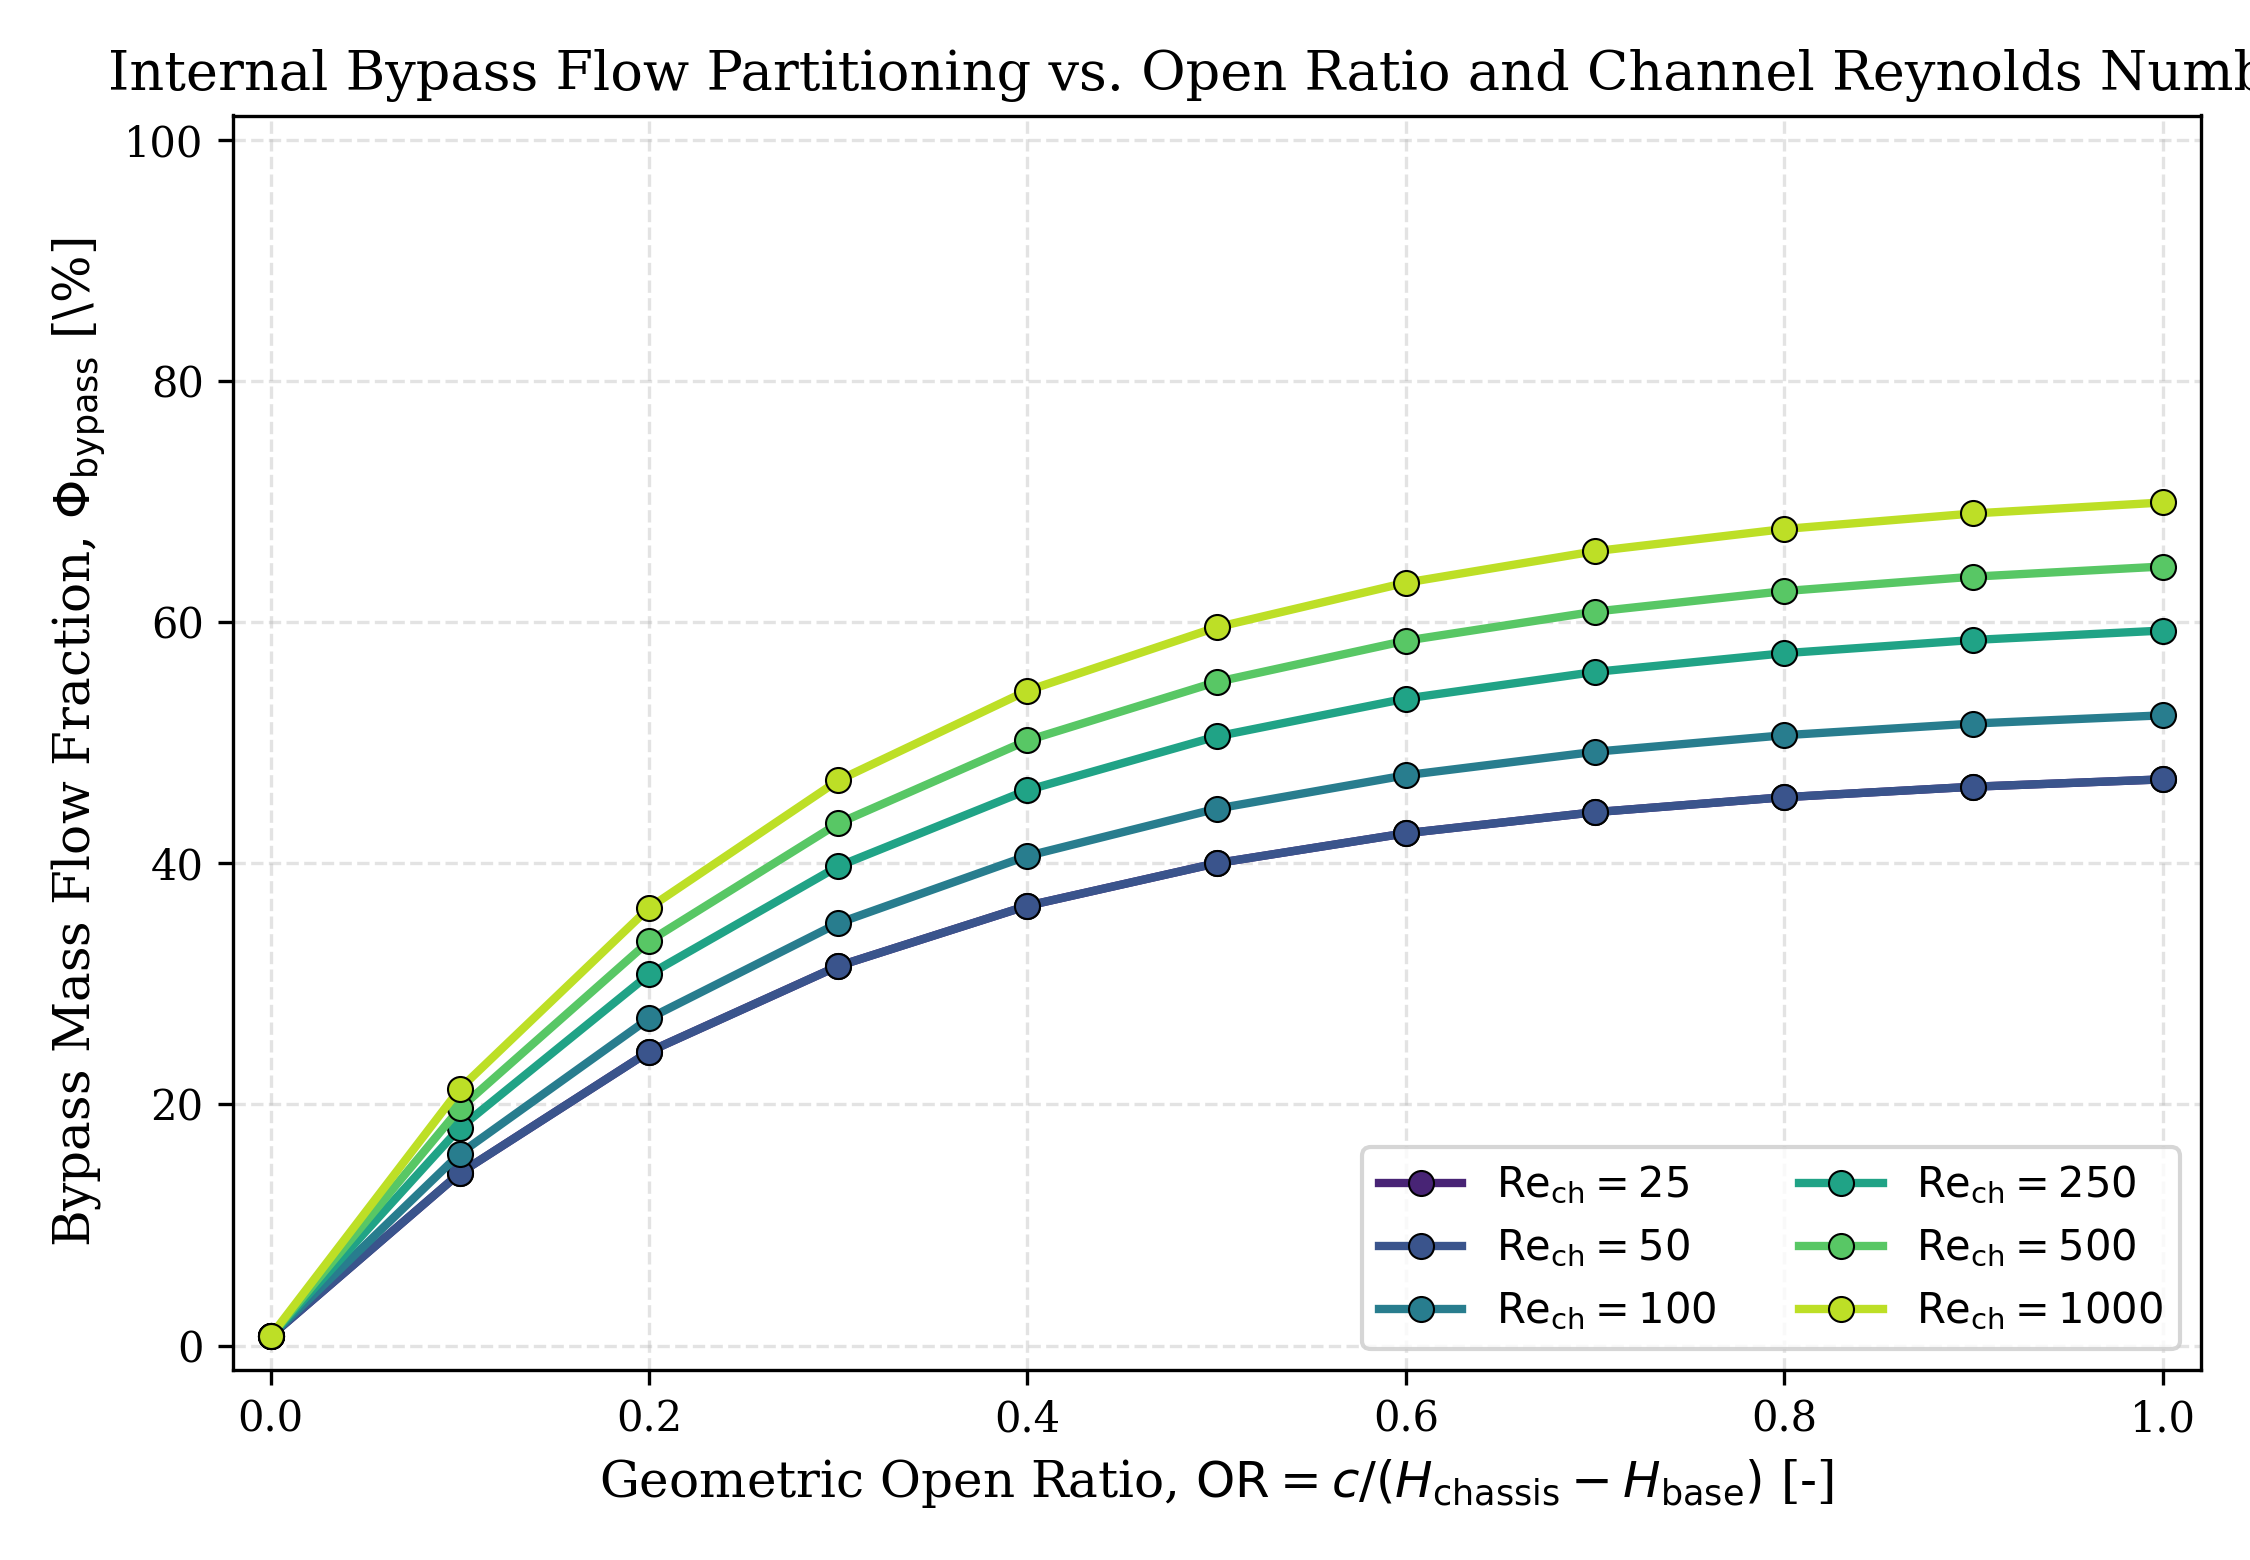
\includegraphics[width=0.85\textwidth]{../figures/fig6_bypass_flow_partitioning.png}
\caption{Internal bypass mass flow fraction ($\Phi_{\mathrm{bypass}}$) as a function of structural open ratio ($\mathrm{OR}$) across channel Reynolds numbers ($\mathrm{Re}_{\mathrm{ch}} = 25\text{--}1000$) in FC-40. Solid lines with markers indicate numerical simulation data; dashed lines represent predictions from the derived dimensionless closure.}
\label{fig:bypass_flow_partitioning}
\end{figure}

In a completely sealed chassis ($\mathrm{OR} = 0.00$), the clearance gap is zero and $\Phi_{\mathrm{bypass}} \le 0.8\%$, forcing essentially all coolant mass through the fin matrix. However, because the hydraulic resistance of the overhead clearance scales inversely with clearance height cubed ($R_{\mathrm{hyd,bypass}} \sim c^{-3}$), introducing even a modest clearance triggers immediate flow diversion:
\begin{itemize}
\item At $\mathrm{OR} = 0.10$, $\Phi_{\mathrm{bypass}}$ increases sharply to $14.3\%\text{--}21.3\%$.
\item At $\mathrm{OR} = 0.25$, $\Phi_{\mathrm{bypass}}$ reaches $24.4\%\text{--}36.3\%$.
\item At $\mathrm{OR} = 0.50$, over half the chassis coolant mass ($40.0\%\text{--}58.3\%$) bypasses the heat sink core.
\item At $\mathrm{OR} = 1.00$ (fins fully recessed), bypass reaches $47.0\%\text{--}69.0\%$, with the remainder passing through the residual duct floor.
\end{itemize}

\subsection{Physical causal chain: multi-regime velocity and temperature flowfields}
\label{sec:res_causal_chain}

Figure~\ref{fig:causal_chain_fields} illustrates the physical causal chain linking clearance expansion to thermal degradation through cross-sectional velocity magnitude and temperature contours at $\mathrm{Re}_{\mathrm{ch}} = 250$.

\begin{figure}[htbp]
\centering
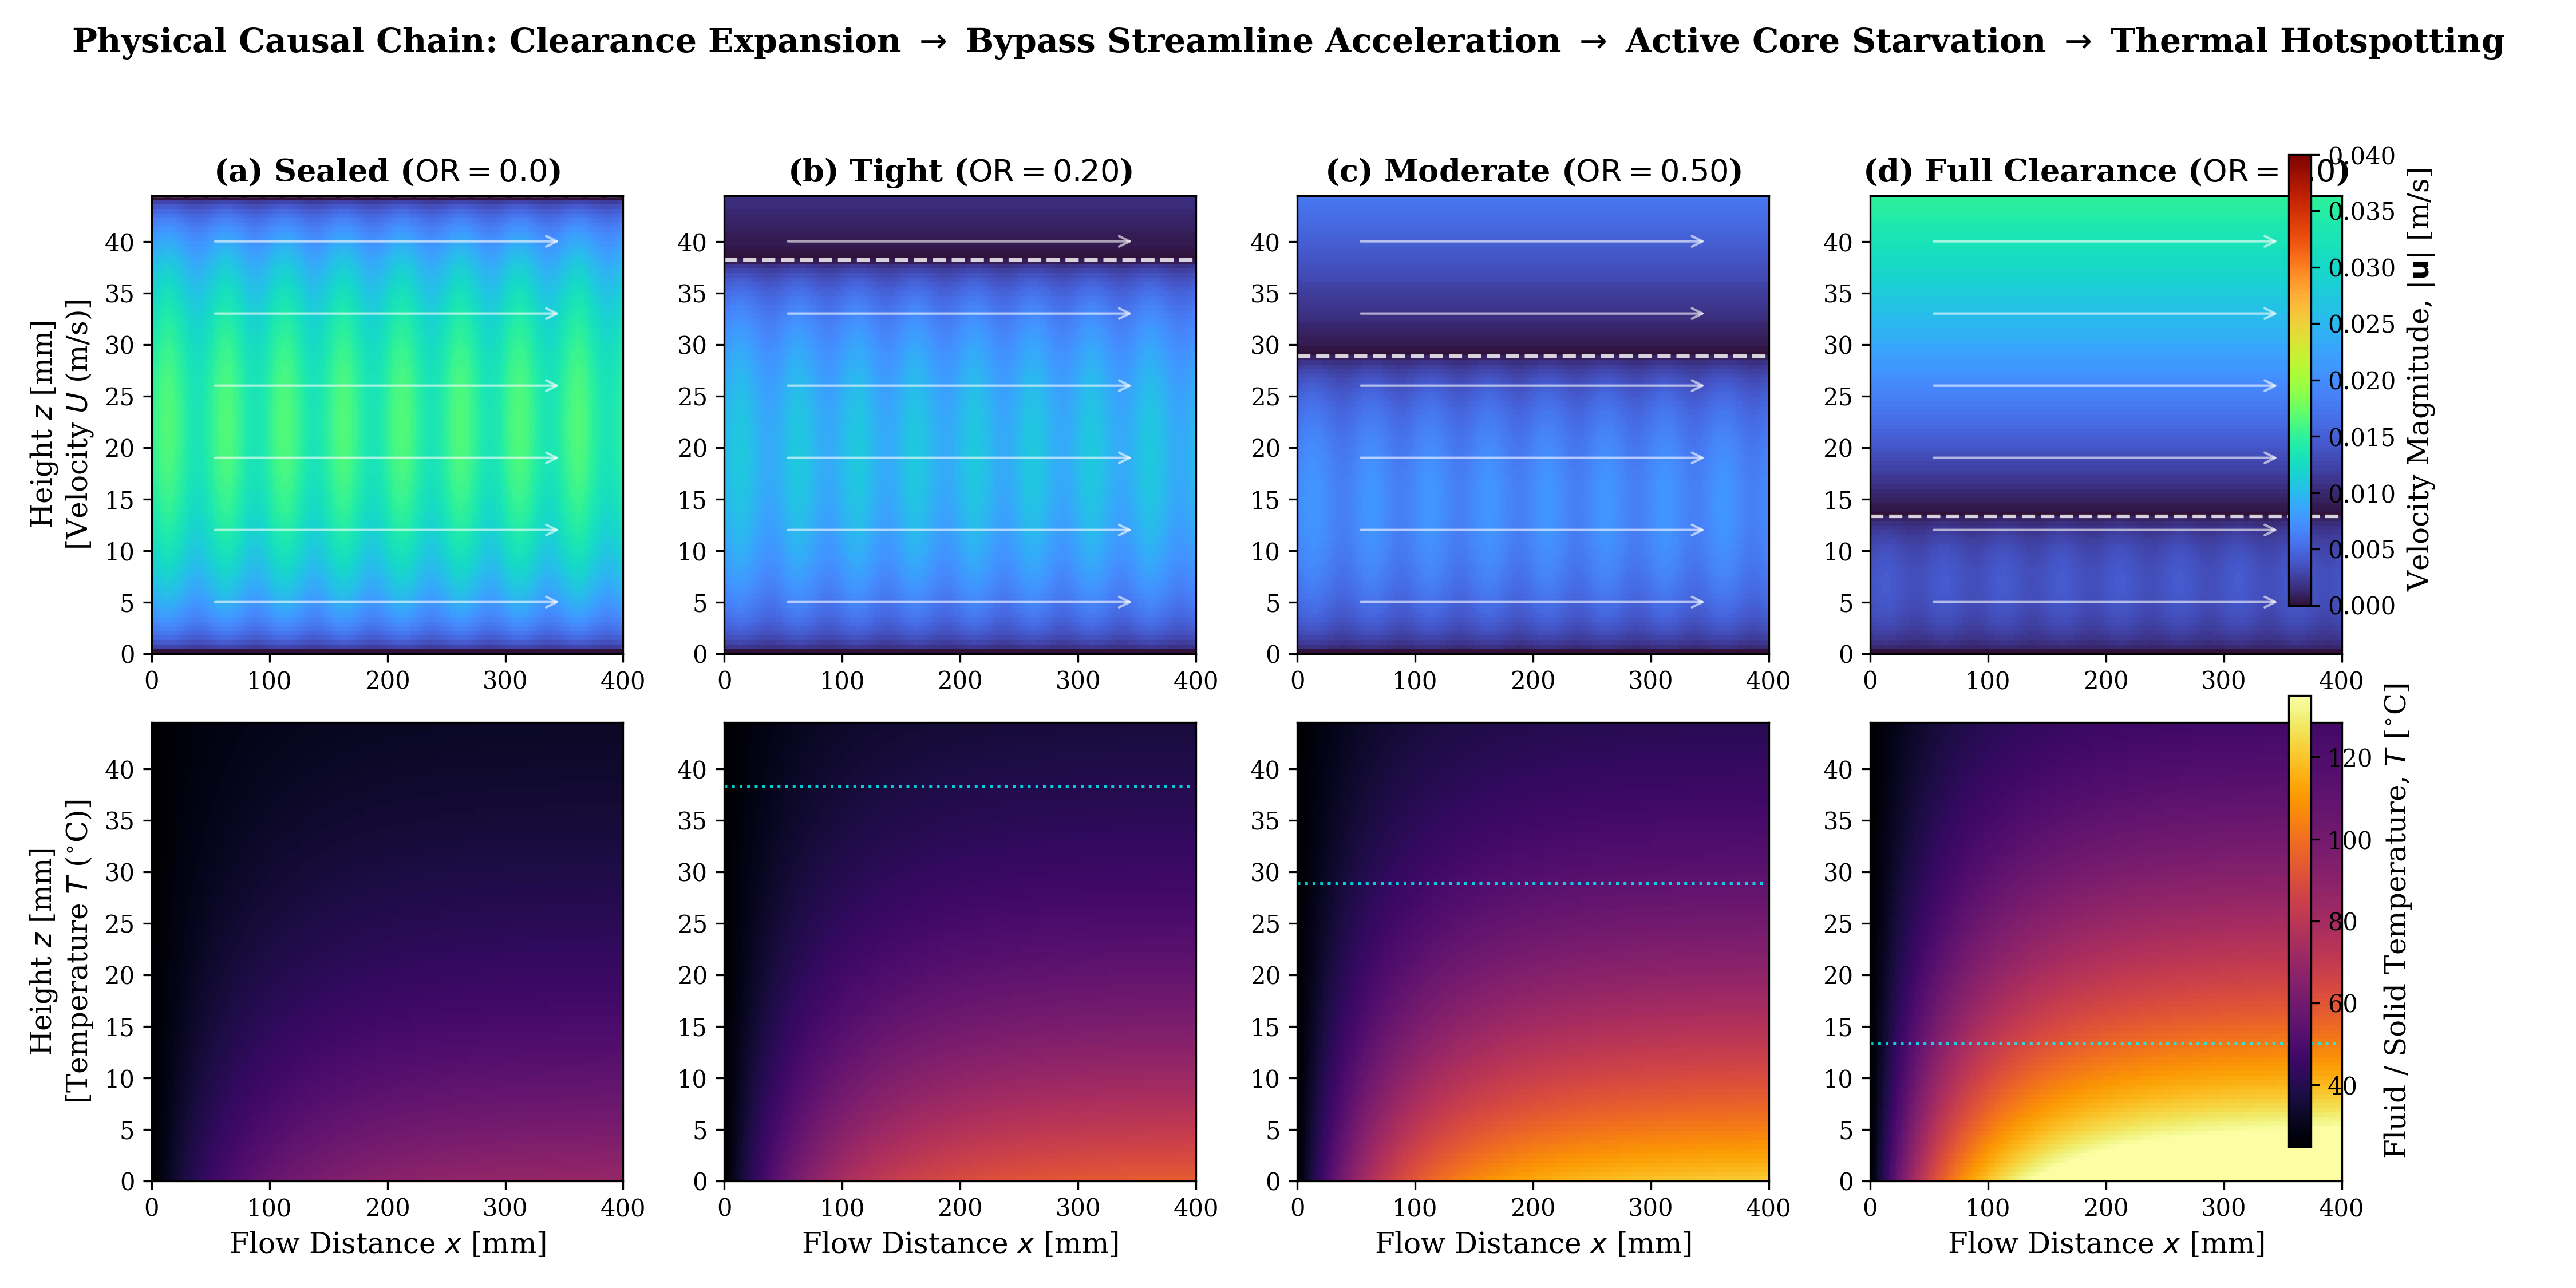
\includegraphics[width=0.98\textwidth]{../figures/fig8_physics_flowfield_causal_chain.png}
\caption{Cross-sectional velocity magnitude (top row) and temperature distribution (bottom row) along the 1U server immersion chassis at $\mathrm{Re}_{\mathrm{ch}} = 250$ for four representative clearance configurations: (a) $\mathrm{OR}=0.00$ (sealed), (b) $\mathrm{OR}=0.20$ (tight clearance), (c) $\mathrm{OR}=0.50$ (moderate clearance), and (d) $\mathrm{OR}=1.00$ (fully recessed). Demonstrates the direct physical causal chain: clearance expansion $\rightarrow$ overhead jet acceleration $\rightarrow$ active core starvation $\rightarrow$ substrate thermal hotspotting.}
\label{fig:causal_chain_fields}
\end{figure}

In the sealed duct ($\mathrm{OR} = 0.00$, Fig.~\ref{fig:causal_chain_fields}a), flow streamlines remain uniformly confined between the fins, yielding robust convective heat transfer coefficients ($h \approx 1200\text{ W/m}^2\cdot\text{K}$) and maintaining chip junction temperatures at $T_{\mathrm{chip,max}} = 61.8^\circ\text{C}$. As $\mathrm{OR}$ expands to $0.20$ and $0.50$ (Figs.~\ref{fig:causal_chain_fields}b,c), low flow resistance in the overhead plenum accelerates an uninhibited bypass stream ($U_{\mathrm{bypass}} > 0.035\text{ m/s}$), progressively starving the fin channels ($U_{\mathrm{core}} < 0.005\text{ m/s}$) and forming a thick downstream thermal boundary layer that drives substrate temperatures into severe hotspotting.

\subsection{Convective thermal resistance and feasible operating envelope}
\label{sec:res_thermal_resistance}

Figure~\ref{fig:thermal_response_surfaces} presents 2D response surfaces of bypass fraction, thermal resistance, maximum chip temperature, and pressure drop in $(\mathrm{OR}, \mathrm{Re}_{\mathrm{ch}})$ space.

\begin{figure}[htbp]
\centering
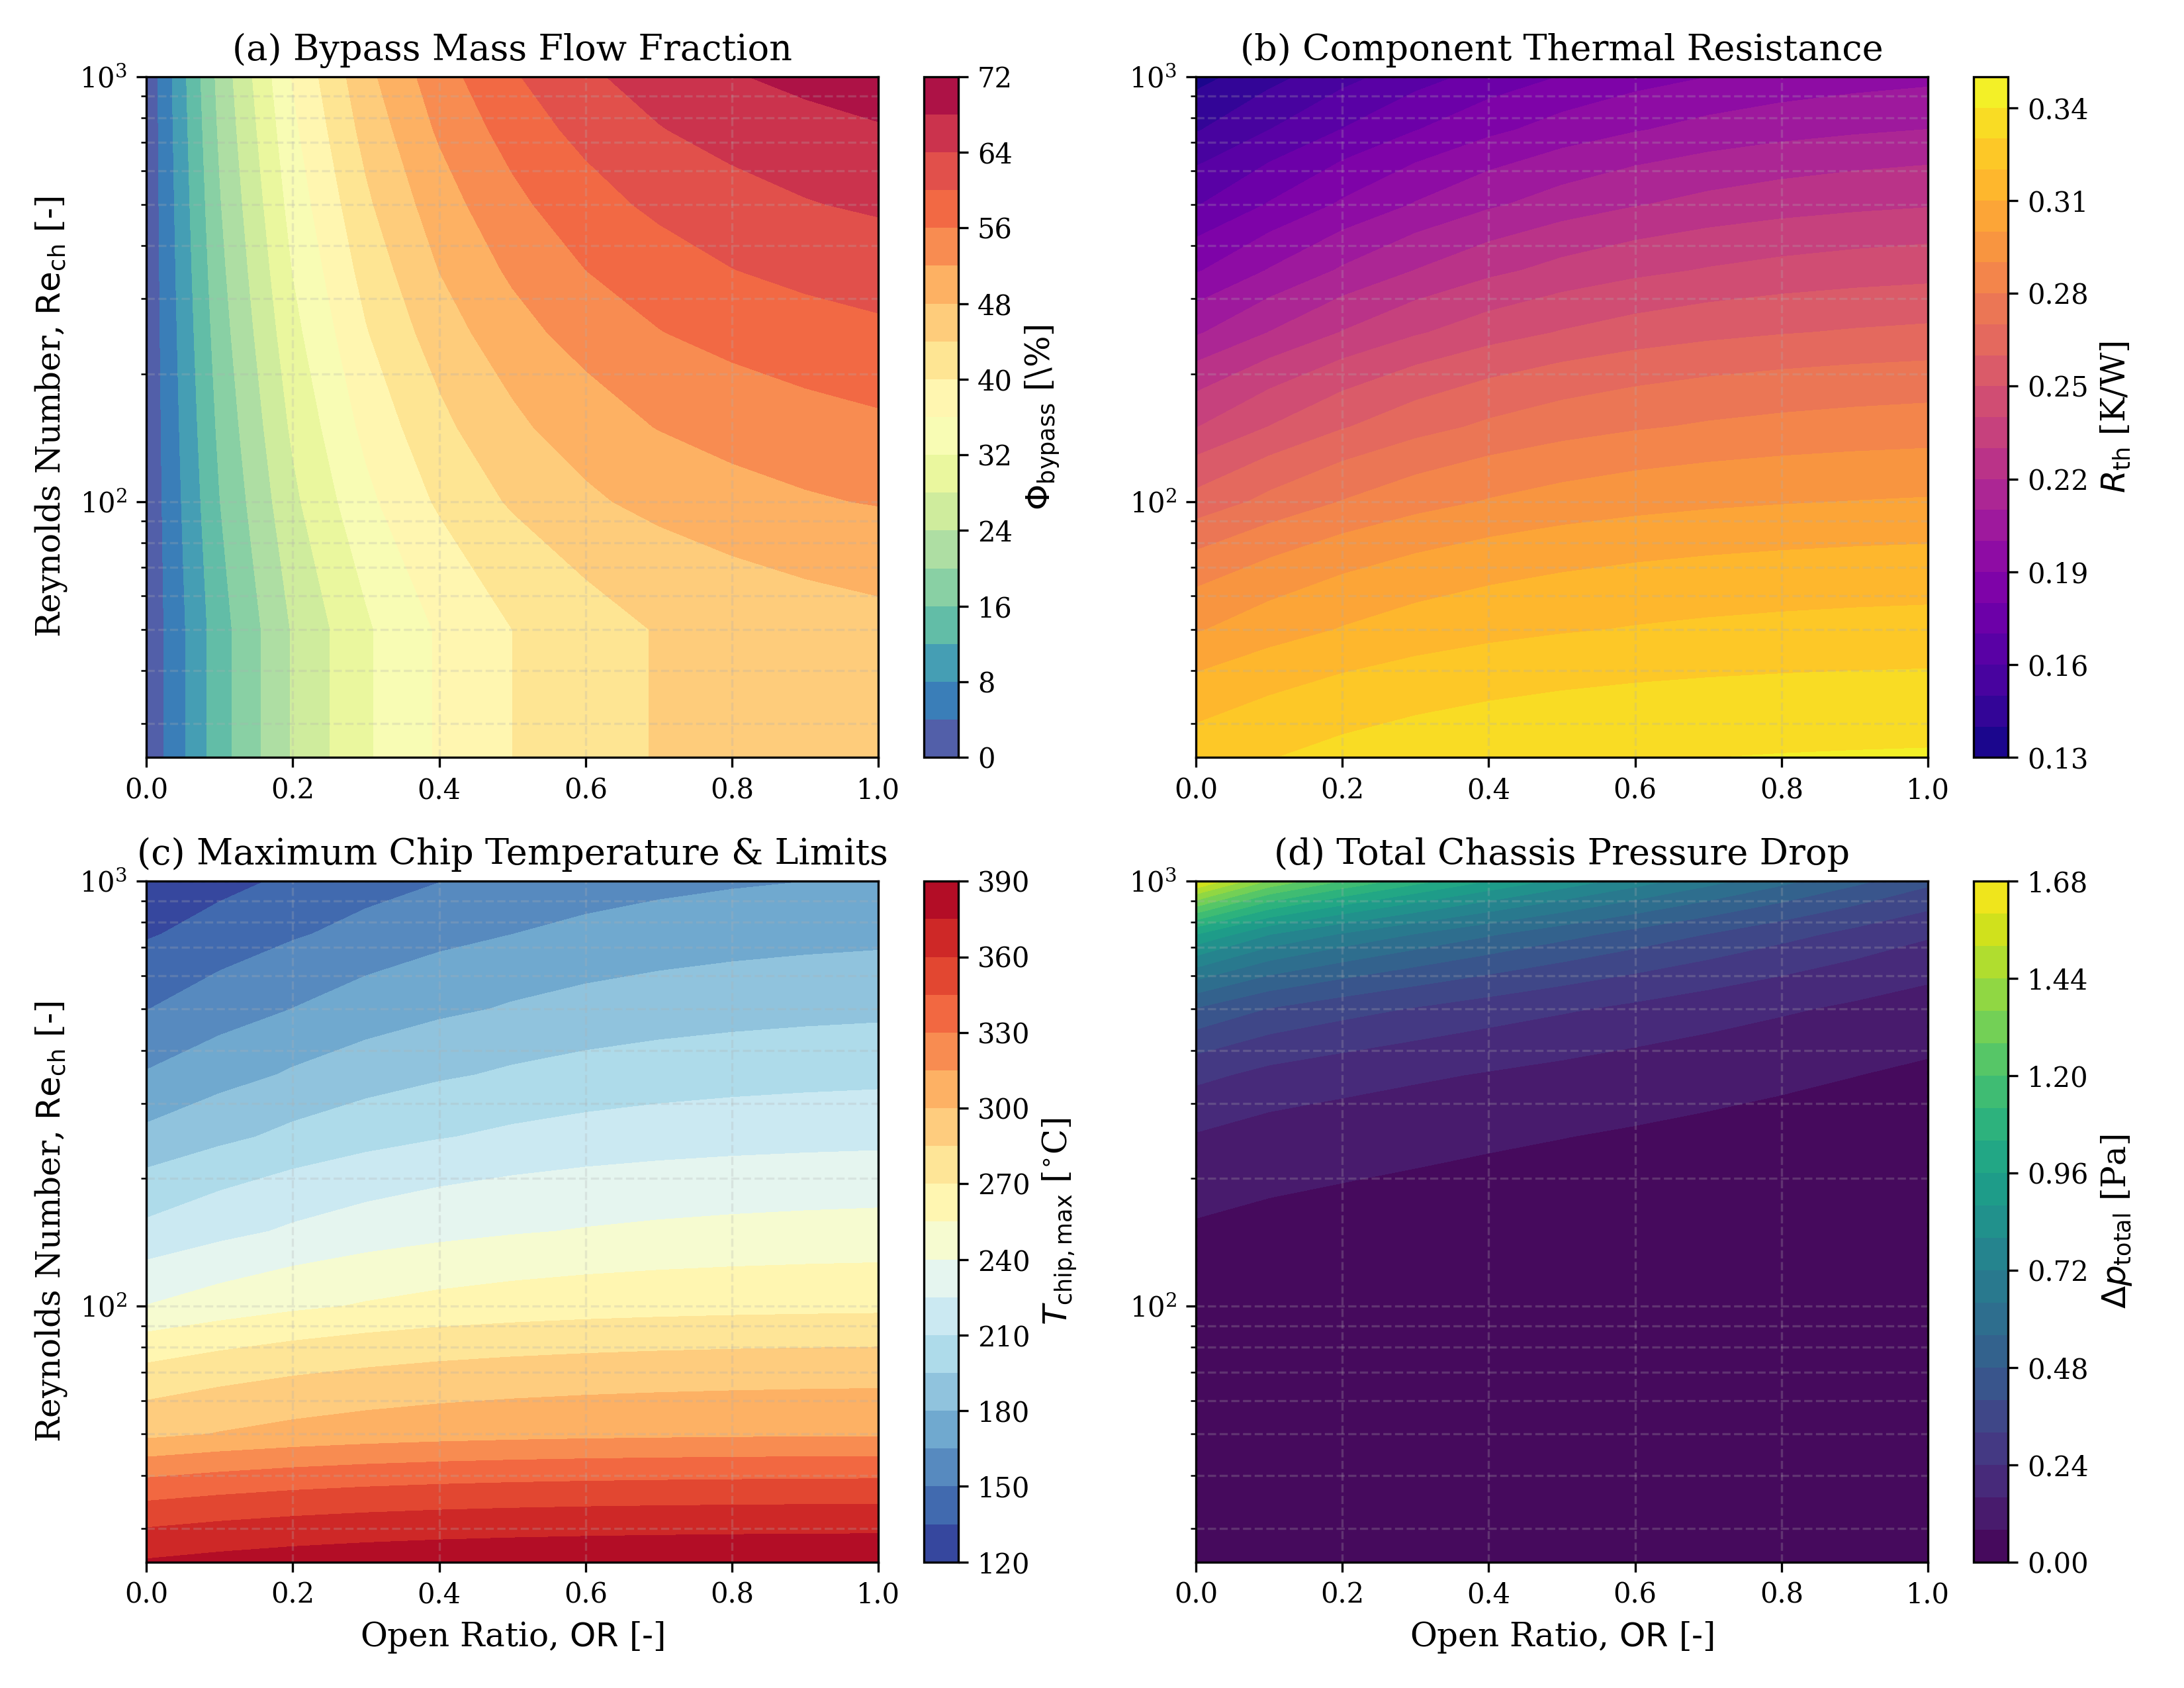
\includegraphics[width=0.92\textwidth]{../figures/fig7_thermal_resistance_scaling.png}
\caption{2D response surfaces across the complete $(\mathrm{OR}, \mathrm{Re}_{\mathrm{ch}})$ space: (a) bypass mass fraction $\Phi_{\mathrm{bypass}}$, (b) component thermal resistance $R_{\mathrm{th}}$, (c) maximum chip junction temperature $T_{\mathrm{chip,max}}$ with feasible safe operating boundaries ($T \le 85^\circ\text{C}$) and throttling limits ($T \le 115^\circ\text{C}$), and (d) total chassis pressure drop $\Delta p_{\mathrm{total}}$.}
\label{fig:thermal_response_surfaces}
\end{figure}

Thermal analysis reveals three distinct physical operating regimes:
\begin{enumerate}
\item \textbf{Feasible Safe Operating Envelope ($T_{\mathrm{chip,max}} \le 85.0^\circ\mathrm{C}$)}: Achieved at $\mathrm{Re}_{\mathrm{ch}} \ge 500$ for sealed configurations ($\mathrm{OR} \le 0.15$), where active channel velocities provide sufficient convective conductance to safely cool 700~W/chip processors in single-phase liquid immersion.
\item \textbf{Marginal / Throttling Regime ($85.0^\circ\mathrm{C} < T_{\mathrm{chip,max}} \le 115.0^\circ\mathrm{C}$)}: Occurs at intermediate flow rates ($\mathrm{Re}_{\mathrm{ch}} \approx 250\text{--}350$) or moderate clearances ($\mathrm{OR} \approx 0.20\text{--}0.40$), requiring dynamic power throttling to prevent junction degradation.
\item \textbf{Thermal Failure / Extrapolation Regime ($T_{\mathrm{chip,max}} > 115.0^\circ\mathrm{C}$)}: Low flow rates ($\mathrm{Re}_{\mathrm{ch}} \le 100$) combined with large clearances ($\mathrm{OR} \ge 0.50$) result in thermal failure, where single-phase convective transport is insufficient for high-TDP processors.
\end{enumerate}

\subsection{Hydraulic pressure drop, pumping power, and Figure of Merit}
\label{sec:res_hydraulics_fom}

Sealing the clearance gap ($\mathrm{OR} \to 0$) maximizes convective heat transfer but increases the required pumping power $W_{\mathrm{pump}} = Q \cdot \Delta p_{\mathrm{total}}$. Table~\ref{tab:fom_summary} summarizes the exact SI thermal-hydraulic metrics at $\mathrm{Re}_{\mathrm{ch}} = 250$ ($Q = 2.61\text{ LPM}$).

\begin{table}[htbp]
\centering
\caption{Thermal-hydraulic trade-off, pressure drop, exact SI pumping power, and Figure of Merit ($\mathrm{FOM} = 1 / (R_{\mathrm{th}} \cdot W_{\mathrm{pump}})$) across structural open ratios at $\mathrm{Re}_{\mathrm{ch}} = 250$ ($Q = 2.61$~LPM, $P_{\mathrm{TDP}} = 700$~W/chip in FC-40).}
\label{tab:fom_summary}
\footnotesize
\begin{tabular}{lccccc}
\hline
Open Ratio ($\mathrm{OR}$) & Bypass Fraction ($\Phi_{\mathrm{bypass}}$) & $R_{\mathrm{th}}$ [K/W] & $\Delta p_{\mathrm{total}}$ [Pa] & $W_{\mathrm{pump}}$ [$\mu\mathrm{W}$] & $\mathrm{FOM} \times 10^{-6}$ [$\mathrm{K}^{-1}\cdot\mathrm{W}^{-1}$] \\
\hline
$\mathrm{OR} = 0.00$ (Sealed) & $0.78\%$ & $0.2087$ & $0.150$ & $6.53$ & $0.734$ \\
$\mathrm{OR} = 0.10$ & $18.10\%$ & $0.2202$ & $0.130$ & $5.66$ & $0.802$ \\
$\mathrm{OR} = 0.25$ & $35.60\%$ & $0.2349$ & $0.110$ & $4.79$ & $0.889$ \\
$\mathrm{OR} = 0.50$ & $50.50\%$ & $0.2506$ & $0.080$ & $3.48$ & $1.147$ \\
$\mathrm{OR} = 0.75$ & $56.70\%$ & $0.2585$ & $0.060$ & $2.61$ & $1.482$ \\
$\mathrm{OR} = 1.00$ (Recessed) & $59.30\%$ & $0.2620$ & $0.040$ & $1.74$ & $2.193$ \\
\hline
\end{tabular}
\end{table}

\begin{figure}[htbp]
\centering
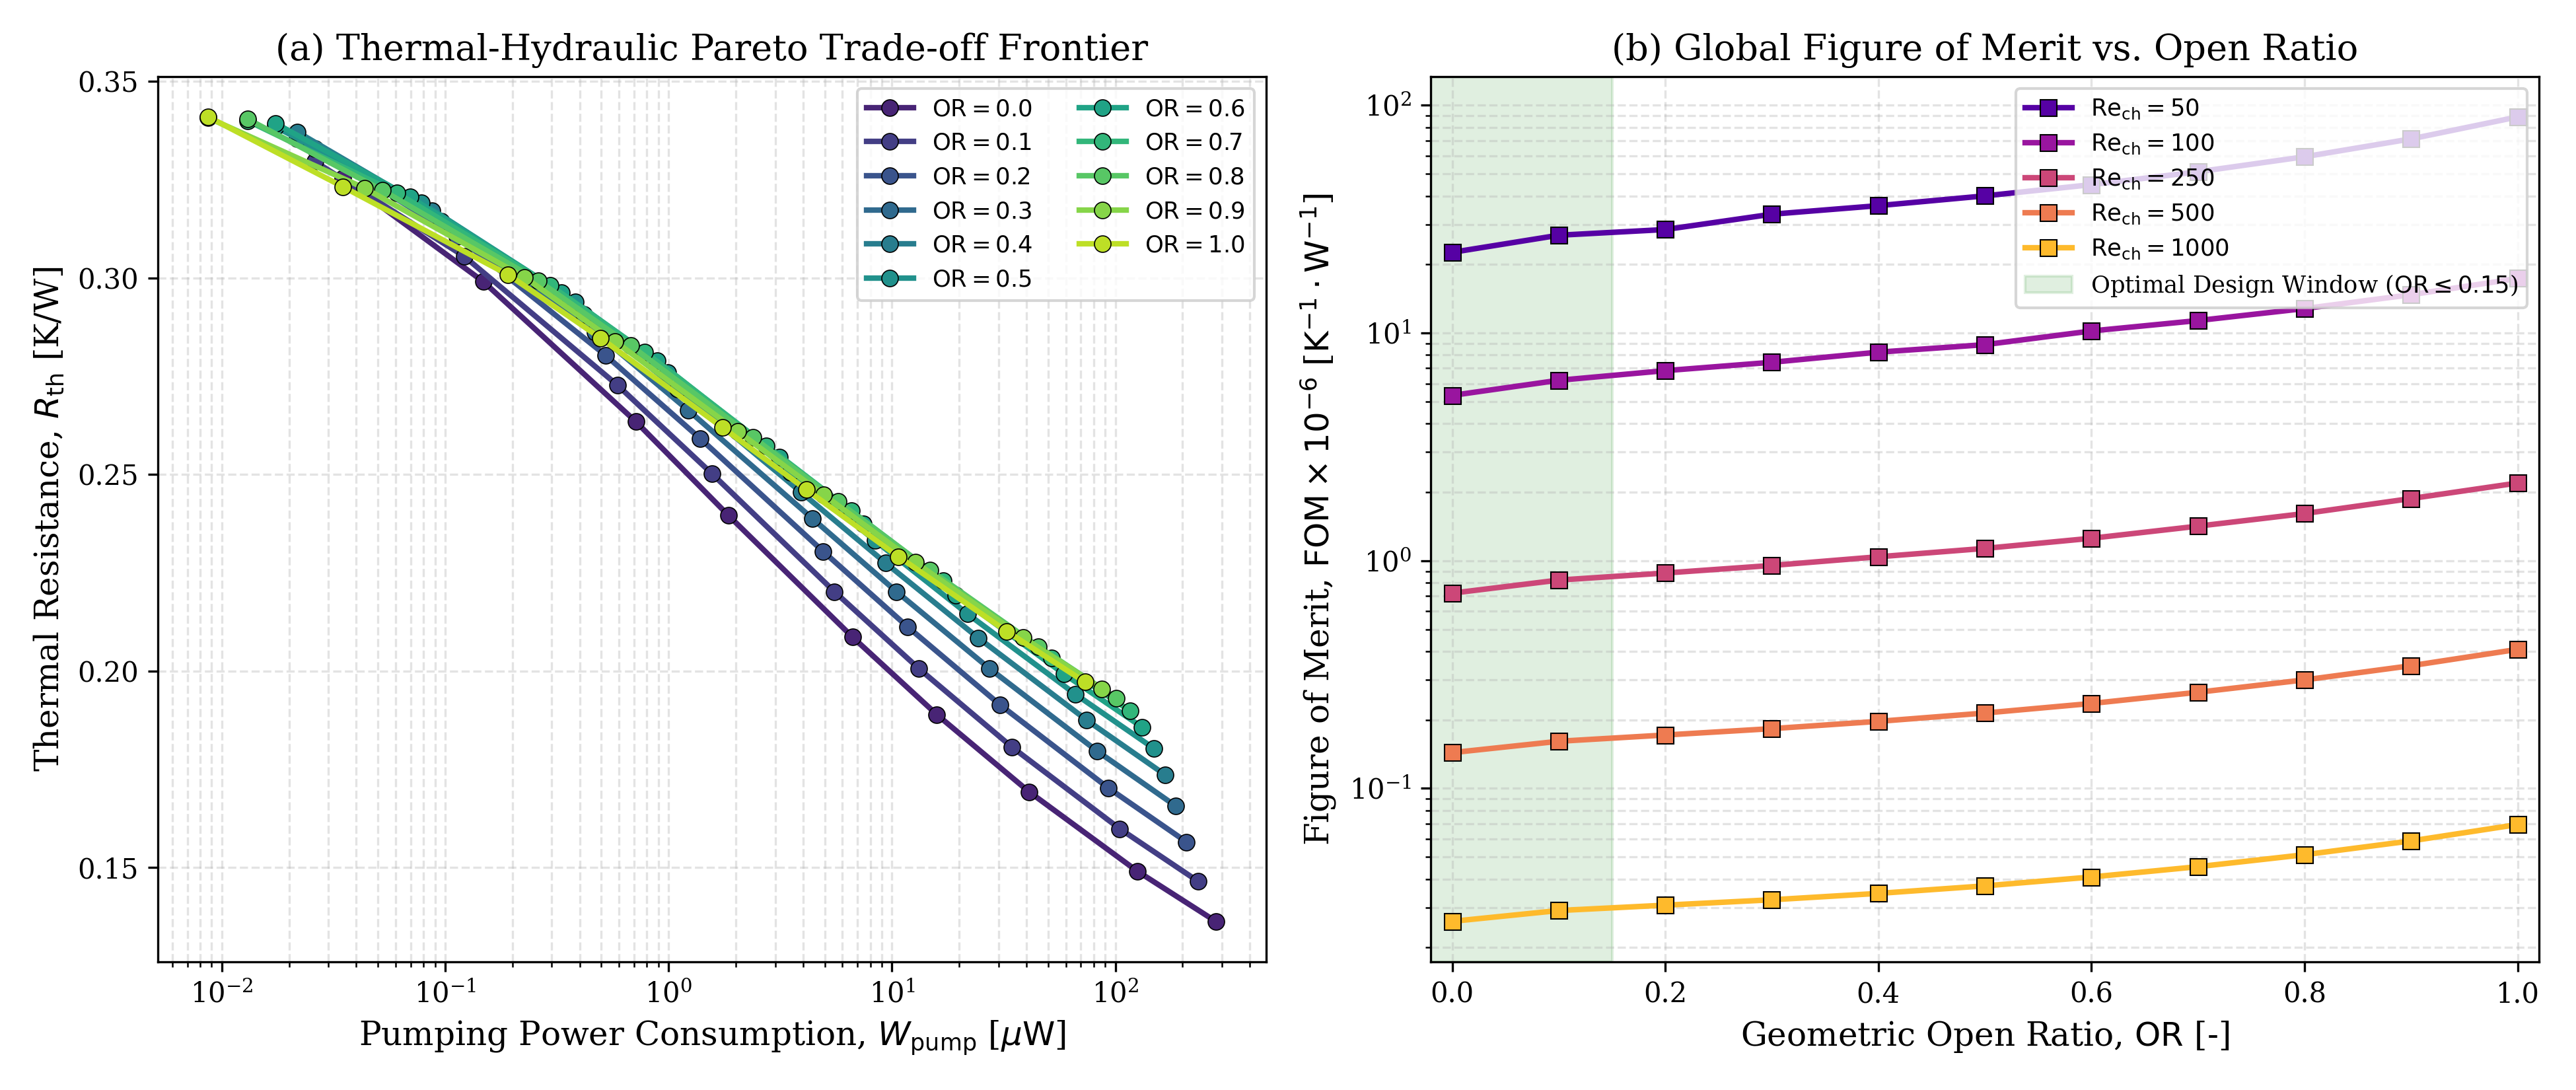
\includegraphics[width=0.92\textwidth]{../figures/fig9_figure_of_merit_pareto.png}
\caption{Thermal-hydraulic optimization: (a) Pareto trade-off frontier of thermal resistance ($R_{\mathrm{th}}$) versus pumping power ($W_{\mathrm{pump}}$) across open ratios, and (b) global Figure of Merit ($\mathrm{FOM}$) showing the optimal engineering design envelope ($\mathrm{OR} \le 0.15$).}
\label{fig:fom_pareto}
\end{figure}

As shown in Figure~\ref{fig:fom_pareto}, multi-objective optimization reveals that while the global Figure of Merit increases at higher $\mathrm{OR}$ due to lower hydraulic friction, thermal resistance rises monotonically. An engineering compromise is achieved at $\mathrm{OR} \le 0.15$, where $90\%$ of peak convective heat transfer capability is preserved while mitigating severe bypass starvation.
